% Copyright (c) 2018 Alexander Bluhm <bluhm@genua.de>
%
% Permission to use, copy, modify, and distribute this software for any
% purpose with or without fee is hereby granted, provided that the above
% copyright notice and this permission notice appear in all copies.
%
% THE SOFTWARE IS PROVIDED "AS IS" AND THE AUTHOR DISCLAIMS ALL WARRANTIES
% WITH REGARD TO THIS SOFTWARE INCLUDING ALL IMPLIED WARRANTIES OF
% MERCHANTABILITY AND FITNESS. IN NO EVENT SHALL THE AUTHOR BE LIABLE FOR
% ANY SPECIAL, DIRECT, INDIRECT, OR CONSEQUENTIAL DAMAGES OR ANY DAMAGES
% WHATSOEVER RESULTING FROM LOSS OF USE, DATA OR PROFITS, WHETHER IN AN
% ACTION OF CONTRACT, NEGLIGENCE OR OTHER TORTIOUS ACTION, ARISING OUT OF
% OR IN CONNECTION WITH THE USE OR PERFORMANCE OF THIS SOFTWARE.

\documentclass[14pt]{beamer}
\usetheme{Frankfurt}
\usepackage{tikz}
\usepackage{graphicx}
\usepackage{tipa}
\usepackage{alltt}
\usepackage{xcolor}
\author{Alexander Bluhm}
\title{OpenBSD Security Features}
\institute{genua GmbH\\ \url{bluhm@genua.de}\\ \url{bluhm@openbsd.org}}
\date{September 20, 2018}
\let\Tiny\tiny

\begin{document}

\begin{frame}
\titlepage
\end{frame}

\begin{frame}{Agenda}
\setcounter{tocdepth}{1}
\tableofcontents
\end{frame}

\section{Malloc}

\subsection{Avoid malloc(3) Overflow}
\begin{frame}{Avoid malloc(3) Overflow}
\begin{itemize}
    \item \texttt{malloc(nmemb * size)}
    \item \texttt{calloc(nmemb, size)}
    \item \texttt{reallocarray(ptr, nmemb, size)}
    \item Libc does overflow check.
\end{itemize}
\end{frame}

\subsection{Clear Sensitive Memory}
\begin{frame}{Clear Sensitive Memory}
\begin{itemize}
    \item \texttt{bzero(buf, len); free(buf)}
    \item \texttt{explicit\_bzero(buf, len)}
    \item \texttt{freezero(ptr, len)}
    \item \texttt{recallocarray(ptr, oldnmemb, nmemb, size)}
    \item Libc does \texttt{memset(3)}.
\end{itemize}
\end{frame}

\subsection{Malloc(3) Options}
\begin{frame}{Malloc(3) Options}
\begin{itemize}
    \item randomize
    \item guard pages
    \item double free check
    \item use after free check
    \item allocate junking
    \item free junking
    \item canaries
    \item unmap pages
\end{itemize}
\end{frame}

\subsection{Random Everywhere}
\begin{frame}{Random Everywhere}
\begin{itemize}
    \item \texttt{arc4random()} ChaCha20
    \item safe \texttt{fork()}
    \item \texttt{getentropy(buf, buflen)}
    \item \texttt{srand[om]\_deterministic(seed)}
    \item \texttt{.openbsd.randomdata} ELF section
    \item /etc/random.seed
    \item /var/db/host.random
\end{itemize}
\end{frame}

\subsection{Random ELF section}
\begin{frame}{Random ELF section}
\begin{itemize}
    \item kernel
    \begin{itemize}
	\item stack protector guard
	\item \texttt{arc4random(9)}
    \end{itemize}
    \item libc
    \begin{itemize}
	\item stack protector guard
	\item \texttt{setjmp(3)/longjmp(3)}
    \end{itemize}
    \item ld.so
    \begin{itemize}
	\item stack protector guard
	\item \texttt{kbind(3) cookie}
    \end{itemize}
\end{itemize}
\end{frame}

\section{Pledge}

\subsection{pledge(2) Motivation}
\begin{frame}{pledge(2) Motivation}
\begin{itemize}
    \item restrict system calls
    \item declare functional requirements
    \item tool for programmer
    \item abort process at violation
    \item log problems or attacks
\end{itemize}
\end{frame}

\subsection{Way to pledge(2)}
\begin{frame}{Way to pledge(2)}
\begin{itemize}
    \item studdy existing programs
    \item pattern initialization and main loop
    \item design classes of promises
    \item reimplement some libc functions
    \item pledge nearly all programs
\end{itemize}
\end{frame}

\subsection{pledge(2) Consequences}
\begin{frame}{pledge(2) Consequences}
\begin{itemize}
    \item cleanup program flow
    \item delete (mis-)features
    \item design security model
\end{itemize}
\end{frame}

\subsection{New System Calls}
\begin{frame}{New System Calls}
\begin{itemize}
    \item \texttt{socket(..., SOCK\_DGRAM \textpipe{} SOCK\_DNS, ...)}
    \item \texttt{sendsyslog("log message", 11, LOG\_CONS)}
    \item \texttt{getentropy(buf, buflen)}
    \item \texttt{kbind(param, psize, cookie)}
\end{itemize}
\end{frame}

\subsection{Use sendsyslog(2)}
\begin{frame}{Use sendsyslog(2)}
\begin{itemize}
    \item \texttt{syslog(3)}, obviously
    \item \texttt{memcpy(3)}
    \item stack protector smash handler
    \item ld.so
\end{itemize}
\end{frame}

\subsection{Lazy Binding}
\begin{frame}{Lazy Binding}
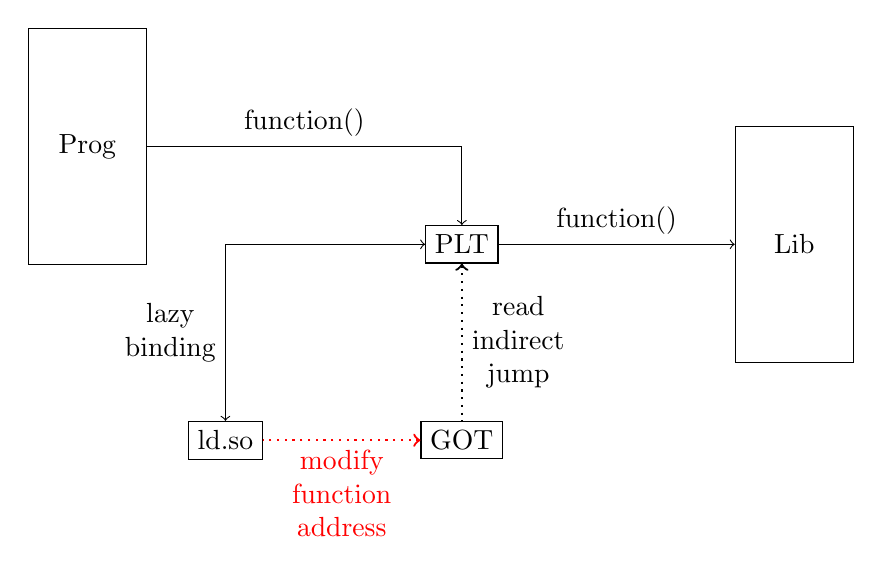
\begin{tikzpicture}
\draw
    node [draw,minimum height=3cm,minimum width=1.5cm] (prog) {Prog};
\draw (prog.east) [->] -- ++(4,0) node [midway,above] {function()} -- ++(0,-1)
    node [draw,below] (plt) {PLT};
\draw (plt.south) [<-,dotted,thick] -- ++(0,-2)
    node [midway,right,align=center] {read\\ indirect\\ jump}
    node [draw,solid,thin,below] (got) {GOT};
in ld.so \draw (got.west) [<-,dotted,thick,red] -- ++(-2,0)
    node [midway,below,align=center] {modify\\ function\\ address}
    node [draw,solid,thin,left,black] (ldso) {ld.so};
\draw (plt.west) [<->] -|
    node [near end,left,align=center] {lazy\\ binding} (ldso);
\draw (plt.east) [->] -- ++(3,0) node [midway,above] {function()}
    node [draw,right,minimum height=3cm,minimum width=1.5cm] (lib) {Lib};
\end{tikzpicture}
\end{frame}

\subsection{kbind(2) System Call}
\begin{frame}{kbind(2) System Call}
\begin{itemize}
    \item Procedure Linkage Table
    \item Global Offset Table
    \item avoid writeable table of code pointers
    \item \texttt{kbind(param, psize, cookie)}
    \item \texttt{struct \_\_kbind \{ kb\_addr; kb\_size; \} param}
\end{itemize}
\end{frame}

\section{Privilege Separation}

\subsection{Privilege Separation in Processes}
\begin{frame}{Privilege Separation in Processes}
\begin{itemize}
    \item identify isolated tasks with high risk
    \item \texttt{socketpair(2)}
    \item \texttt{fork(2)}
    \item \texttt{chroot(2)}
    \item \texttt{setuid(2)}
    \item \texttt{pledge(2)}
    \item \texttt{imsg\_init(3)}
    \item file descriptor passing
\end{itemize}
\end{frame}

\subsection{Programs with Privsep}
\begin{frame}{Programs with Privsep}
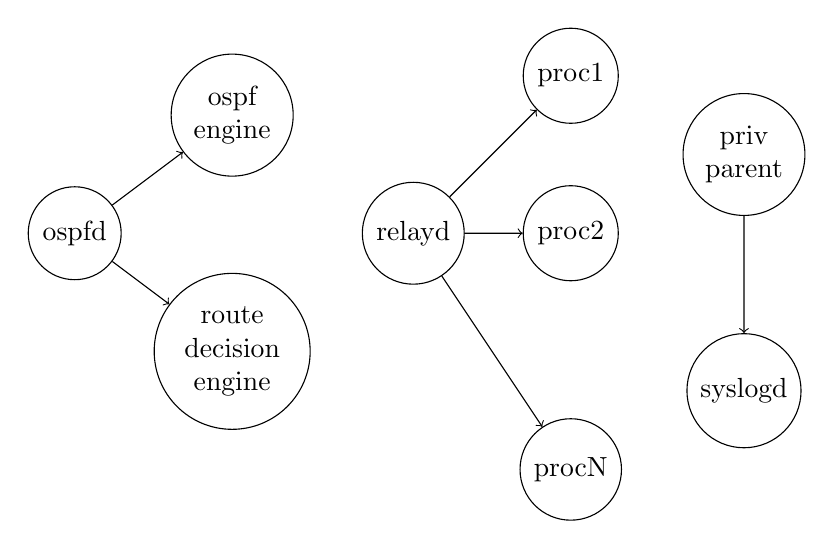
\begin{tikzpicture}
\draw [grow=right,level distance=2cm,sibling distance=3cm]
    (0,0) node [draw,circle,align=center] (ospfd) {ospfd}
    [edge from parent/.style={draw,->}]
    child { node [draw,circle,align=center] (rde) {route\\ decision\\ engine} }
    child { node [draw,circle,align=center] (ospfe) {ospf\\ engine} };
\draw [grow'=right,level distance=2cm,sibling distance=2cm]
    (4.3,0) node [draw,circle,align=center] (relayd) {relayd}
    [edge from parent/.style={draw,->}]
    child { node [draw,circle,align=center] (proc1) {proc1} }
    child { node [draw,circle,align=center] (proc2) {proc2} }
    child { node [draw,circle,align=center,yshift=-1cm] (procn) {procN} };
\draw [grow=down,level distance=3cm]
    (8.5,1) node [draw,circle,align=center] (parent) {priv\\ parent}
    [edge from parent/.style={draw,->}]
    child { node [draw,circle,align=center] (syslogd) {syslogd} };
\end{tikzpicture}
\end{frame}

\subsection{Avoid File Descriptor Exhaustion}
\begin{frame}{Avoid File Descriptor Exhaustion}
\begin{itemize}
    \item \texttt{getdtablecount(2)}
    \item \texttt{getdtablesize(2)}
    \item \texttt{\#define FD\_RESERVE 5}
\end{itemize}
\end{frame}

\section{Buffer Overflow}

\subsection{Stack Buffer Overflow}
\begin{frame}{Stack Buffer Overflow}
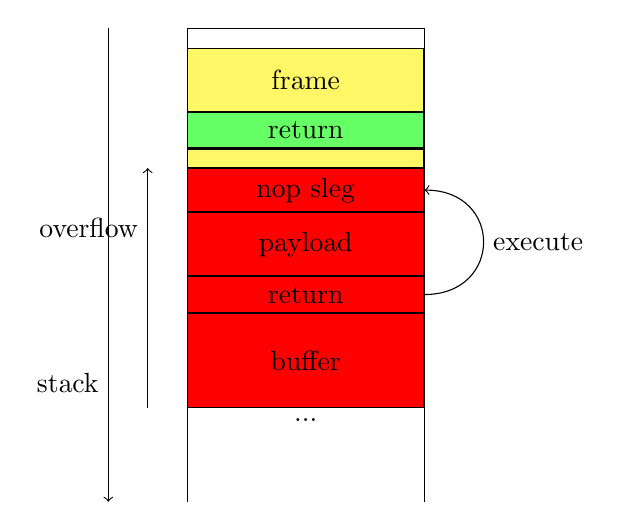
\begin{tikzpicture}
\path
    [minimum width=3cm,below]
    (0,0) node [minimum height=6cm] (stack) {};
\draw
    (stack.south west) -- (stack.north west) --
    (stack.north east) -- (stack.south east);
\path
    [minimum width=3cm,below]
    (stack.north) node (gap) {}
    (gap.south) node [draw,fill=yellow!60,minimum height=.8cm] (frame2) {frame}
    (frame2.south) node [draw,fill=green!60] (return1) {return}
    (return1.south) node [draw,fill=yellow!60,minimum height=0.1cm] (frame1) {}
    (frame1.south) node [draw,fill=red] (nop) {nop sleg}
    (nop.south) node [draw,fill=red,minimum height=0.8cm] (payload) {payload}
    (payload.south) node [draw,fill=red] (return) {return}
    (return.south) node [draw,fill=red,minimum height=1.2cm] (buffer) {buffer}
    (buffer.south) node {...};
\draw
    (stack.north west) +(-1,0) coordinate (sstart)
    (stack.south west) +(-1,0) coordinate (send)
    [->] (sstart) -- (send) node [near end,left] {stack};
\draw
    (buffer.south west) +(-0.5,0) coordinate (bstart)
    (frame1.south west) +(-0.5,0) coordinate (bend)
    [->] (bstart) -- (bend) node [near end,left] {overflow};
\draw [->] (return.east) .. controls +(1,0) and +(1,0) .. (nop.east)
    node [anchor=west,midway] {execute};
\end{tikzpicture}
\end{frame}

\subsection{Stack Protector}
\begin{frame}{Stack Protector}
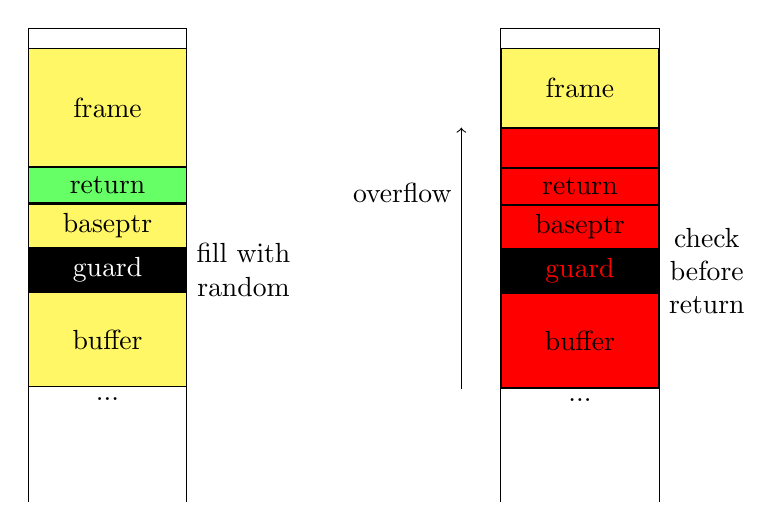
\begin{tikzpicture}
\path
    [minimum width=2cm,below]
    (0,0) node [minimum height=6cm] (stack) {};
\draw
    (stack.south west) -- (stack.north west) --
    (stack.north east) -- (stack.south east);
\path
    [minimum width=2cm,below]
    (stack.north) node (gap) {}
    (gap.south) node [draw,fill=yellow!60,minimum height=1.5cm] (frame) {frame}
    (frame.south) node [draw,fill=green!60] (return) {return}
    (return.south) node [draw,fill=yellow!60] (base) {baseptr}
    (base.south) node [draw,text=white,fill=black] (guard) {guard}
    (guard.south) node [draw,fill=yellow!60,minimum height=1.2cm] (buffer)
	{buffer}
    (buffer.south) node {...};
\path
    (guard.east) node [anchor=west,align=center] {fill with\\ random};

\path
    [minimum width=2cm,below]
    (6,0) node [minimum height=6cm] (stack) {};
\draw
    (stack.south west) -- (stack.north west) --
    (stack.north east) -- (stack.south east);
\path
    [minimum width=2cm,below]
    (stack.north) node (gap) {}
    (gap.south) node [draw,fill=yellow!60,minimum height=1cm] (frame) {frame}
    (frame.south) node [draw,fill=red,minimum height=.5cm] (overflow) {}
    (overflow.south) node [draw,fill=red] (return) {return}
    (return.south) node [draw,fill=red] (base) {baseptr}
    (base.south) node [draw,text=red,fill=black] (guard) {guard}
    (guard.south) node [draw,fill=red,minimum height=1.2cm] (buffer) {buffer}
    (buffer.south) node {...};
\draw
    (buffer.south west) +(-0.5,0) coordinate (bstart)
    (frame.south west) +(-0.5,0) coordinate (bend)
    [->] (bstart) -- (bend) node [near end,left] {overflow};
\path
    (guard.east) node [anchor=west,align=center] {check\\ before\\ return};
\end{tikzpicture}
\end{frame}

\subsection{Page Protection}
\begin{frame}{Page Protection}
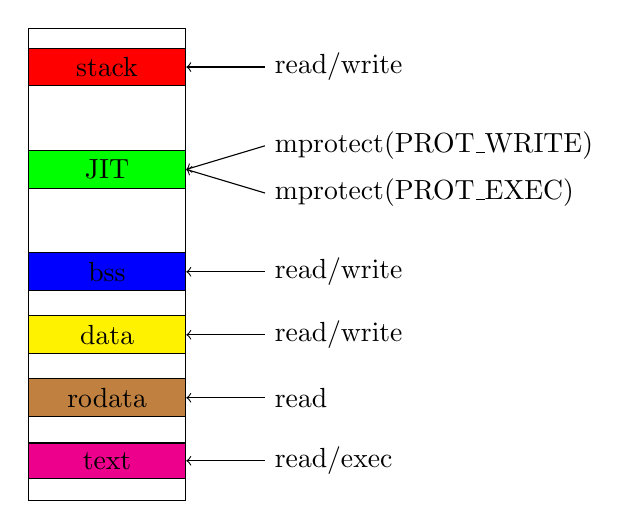
\begin{tikzpicture}
\path
    (0,0) node [draw,below,minimum width=2cm,minimum height=6cm] (proc) {}
    +(0,-0.5) node [draw,minimum width=2cm,fill=red] (stack) {stack}
    +(0,-1.8) node [draw,minimum width=2cm,fill=green] (jit) {JIT}
    +(0,-3.1) node [draw,minimum width=2cm,fill=blue] (bss) {bss}
    +(0,-3.9) node [draw,minimum width=2cm,fill=yellow] (data) {data}
    +(0,-4.7) node [draw,minimum width=2cm,fill=brown] (rodata) {rodata}
    +(0,-5.5) node [draw,minimum width=2cm,fill=magenta] (text) {text};
\draw (stack.east) [<-] -- +(1,0) node [anchor=west] {read/write};
\draw (jit.east) +(1,0) node [anchor=south west] (mwrite)
    {mprotect(PROT\_WRITE)} (mwrite.west) [->] -- (jit.east);
\draw (jit.east) +(1,0) node [anchor=north west] (mexec)
    {mprotect(PROT\_EXEC)} (mexec.west) [->] -- (jit.east);
\draw (bss.east) [<-] -- +(1,0) node [anchor=west] {read/write};
\draw (data.east) [<-] -- +(1,0) node [anchor=west] {read/write};
\draw (rodata.east) [<-] -- +(1,0) node [anchor=west] {read};
\draw (text.east) [<-] -- +(1,0) node [anchor=west] {read/exec};
\end{tikzpicture}
\end{frame}

\subsection{W\^{}X Write Xor Execute}
\begin{frame}{W\^{}X Write Xor Execute}
\begin{itemize}
    \item ld -z wxneeded
    \item mount -o wxallowed
    \item \texttt{mprotect(..., PROT\_WRITE \textpipe{} PROT\_EXEC)}
    \item \texttt{mmap(..., PROT\_WRITE \textpipe{} PROT\_EXEC, ...)}
    \item sysctl kern.wxabort=1
\end{itemize}
\end{frame}

\section{ROP}

\subsection{ROP Return Oriented Programming}
\begin{frame}{ROP Return Oriented Programming}
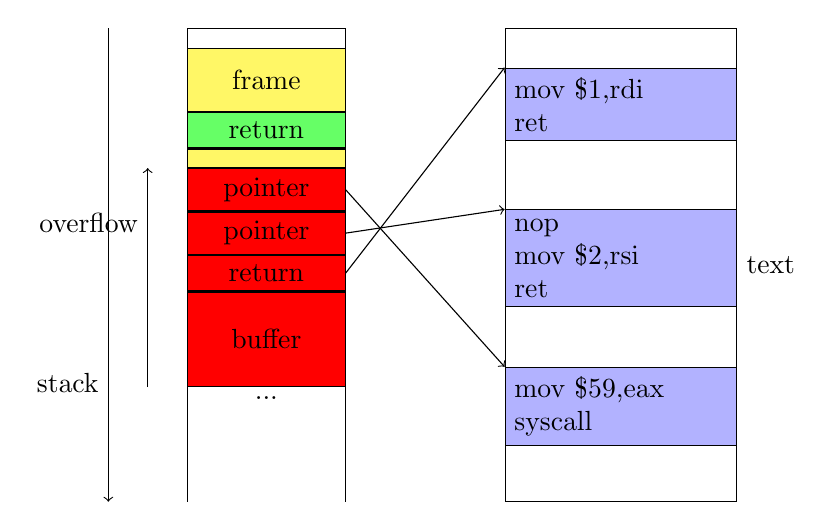
\begin{tikzpicture}
\path
    [minimum width=2cm,below]
    (0,0) node [minimum height=6cm] (stack) {};
\draw
    (stack.south west) -- (stack.north west) --
    (stack.north east) -- (stack.south east);
\path
    [minimum width=2cm,below]
    (stack.north) node (gap) {}
    (gap.south) node [draw,fill=yellow!60,minimum height=.8cm] (frame2) {frame}
    (frame2.south) node [draw,fill=green!60] (return1) {return}
    (return1.south) node [draw,fill=yellow!60,minimum height=0.1cm] (frame1) {}
    (frame1.south) node [draw,fill=red] (pointer2) {pointer}
    (pointer2.south) node [draw,fill=red] (pointer1) {pointer}
    (pointer1.south) node [draw,fill=red] (return) {return}
    (return.south) node [draw,fill=red,minimum height=1.2cm] (buffer) {buffer}
    (buffer.south) node {...};
\draw
    (stack.north west) +(-1,0) coordinate (sstart)
    (stack.south west) +(-1,0) coordinate (send)
    [->] (sstart) -- (send) node [near end,left] {stack};
\draw
    (buffer.south west) +(-0.5,0) coordinate (bstart)
    (frame1.south west) +(-0.5,0) coordinate (bend)
    [->] (bstart) -- (bend) node [near end,left] {overflow};

\path
    [text width=2.7cm,below,align=left]
    (4.5,0) node [draw,minimum height=6cm] (text) {}
    +(0,-0.5) node [draw,fill=blue!30] (gadget0) {mov \$1,rdi\\ ret}
    +(0,-2.3) node [draw,fill=blue!30] (gadget1) {nop\\ mov \$2,rsi\\ ret}
    +(0,-4.3) node [draw,fill=blue!30] (gadget2) {mov \$59,eax\\ syscall};
\draw (text.east) node [anchor=west] {text};
\draw [->] (return.east) -- (gadget0.north west);
\draw [->] (pointer1.east) -- (gadget1.north west);
\draw [->] (pointer2.east) -- (gadget2.north west);
\end{tikzpicture}
\end{frame}

\subsection{Trap Sledge}
\begin{frame}[fragile]{Trap Sledge}
\begin{alltt}
40d435: \textcolor{red}{cc}           int3
40d436: \textcolor{red}{cc}           int3
......
40d43e: \textcolor{red}{cc}           int3
40d43f: \textcolor{red}{cc}           int3
40d440: 55           push %rbp
40d441: 48 89 e5     mov  %rsp,%rbp
40d444: 48 8b 45 10  mov  0x10(%rbp),%rax
40d448: 48 8b 55 18  mov  0x18(%rbp),%rdx
40d44c: 5d           pop  %rbp
40d44d: c3           retq
\end{alltt}
\end{frame}

\subsection{0xc3 Return from Anywhere}
\begin{frame}[fragile]{0xc3 Return from Anywhere}
\begin{itemize}
    \item objdump -d /usr/bin/clang
\end{itemize}
\begin{alltt}
4022ff: 48 83 c0 \textcolor{blue}{08}  add  $0x8,%rax
402303: \textcolor{blue}{48 39} \textcolor{red}{c3}     cmp  %rax,%rbx
402306: 75 ed        jne  4022f5
\end{alltt}
\begin{itemize}
    \item objdump -d --start-address=0x402302 /usr/bin/clang
\end{itemize}
\begin{alltt}
402302: \textcolor{blue}{08 48 39}     or   %cl,0x39(%rax)
402305: \textcolor{red}{c3}           retq
\end{alltt}
\end{frame}

\subsection{Avoid RBX Register}
\begin{frame}[fragile]{Avoid RBX Register}
\begin{itemize}
    \item LLVM compiler patch
\end{itemize}
\begin{alltt}
-EAX,ECX,EDX,ESI,EDI,\textcolor{red}{EBX},EBP,ESP,
-R8D,R9D,R10D,R11D,R14D,R15D,R12D,R13D
+EAX,ECX,EDX,ESI,EDI,R8D,R9D,R10D,
+R11D,R14D,R15D,R12D,R13D,\textcolor{red}{EBX},EBP,ESP
\end{alltt}
\begin{alltt}
 RAX,RCX,RDX,RSI,RDI,R8,R9,R10,R11,
-\textcolor{red}{RBX},R14,R15,R12,R13,RBP,RSP,RIP
+R14,R15,R12,R13,\textcolor{red}{RBX},RBP,RSP,RIP
\end{alltt}
\end{frame}

\subsection{ASLR Address Space Layout Randomization}
\begin{frame}{ASLR Address Space Layout Randomization}
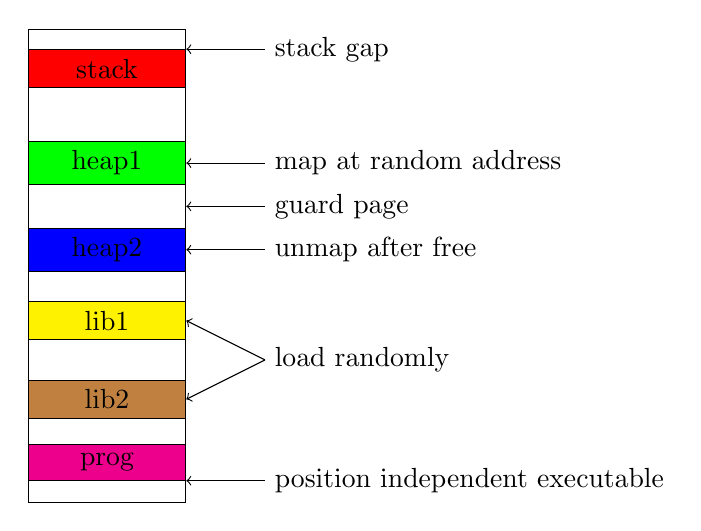
\begin{tikzpicture}
\path
    (0,0) node [draw,below,minimum width=2cm,minimum height=6cm] (proc) {}
    +(0,-0.5) node [draw,minimum width=2cm,fill=red] (stack) {stack}
    +(0,-1.7) node [draw,minimum width=2cm,fill=green] (heap1) {heap1}
    +(0,-2.8) node [draw,minimum width=2cm,fill=blue] (heap2) {heap2}
    +(0,-3.7) node [draw,minimum width=2cm,fill=yellow] (lib1) {lib1}
    +(0,-4.7) node [draw,minimum width=2cm,fill=brown] (lib2) {lib2}
    +(0,-5.5) node [draw,minimum width=2cm,fill=magenta] (prog) {prog};
\draw (stack.north east) [<-] -- +(1,0) node [anchor=west] {stack gap};
\draw (heap1.east) [<-] -- +(1,0) node [anchor=west] {map at random address};
\path (heap1.east) -- (heap2.east) coordinate [midway] (heap);
\draw (heap) [<-] -- +(1,0) node [anchor=west] {guard page};
\draw (heap2.east) [<-] -- +(1,0) node [anchor=west] {unmap after free};
\path (lib1.east) -- (lib2.east) coordinate [midway] (lib)
    (lib) +(1,0) node [anchor=west] (ldso) {load randomly};
\draw (lib1.east) [<-] -- (ldso.west);
\draw (lib2.east) [<-] -- (ldso.west);
\draw (prog.south east) [<-] -- +(1,0) node [anchor=west]
    {position independent executable};
\end{tikzpicture}
\end{frame}

\section{BROP}

\subsection{BROP Blind Return Oriented Programming}
\begin{frame}{BROP Blind Return Oriented Programming}
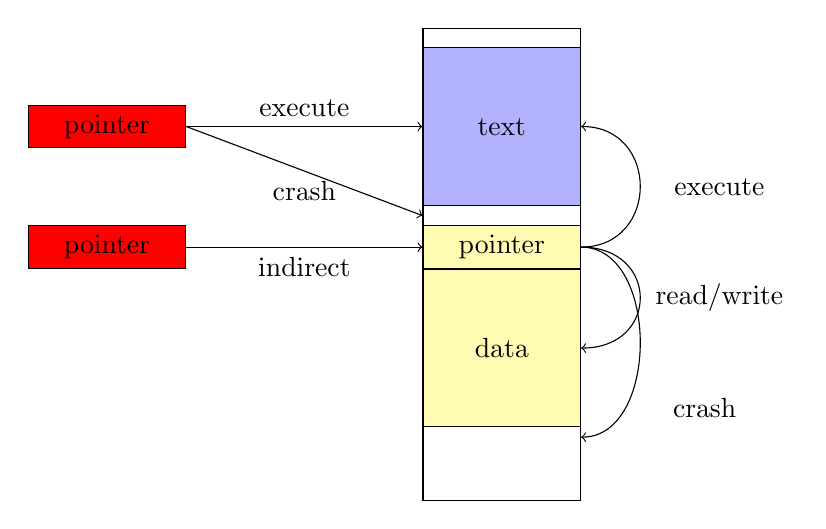
\begin{tikzpicture}
    [minimum width=2cm]
\path
    (0,0) node [draw,minimum height=6cm] (memory) {}
    [below]
    (memory.north) node (gap1) {}
    (gap1.south) node [draw,minimum height=2cm,fill=blue!30] (text) {text}
    (text.south) node (gap2) {}
    (gap2.south) node [draw,,fill=yellow!30] (pointer) {pointer}
    (pointer.south) node [draw,minimum height=2cm,fill=yellow!30] (data) {data}
    (data.south) node (gap3) {};
\draw [<-] (text.west) -- node [midway,above] {execute}
    +(-3,0) node [left,draw,fill=red,minimum width=2cm] (pexe) {pointer};
\draw [->] (pexe.east) -- (gap2.west) node [midway,below] {crash};
\draw [<-] (pointer.west) -- node [midway,below] {indirect}
    +(-3,0) node [left,draw,fill=red,minimum width=2cm] (pind) {pointer};
\draw [->] (pointer.east) .. controls +(1,0) and +(1,0) .. (text.east)
    node [anchor=west,midway] {execute};
\draw [->] (pointer.east) .. controls +(1,0) and +(1,0) .. (data.east)
    node [anchor=west,midway] {read/write};
\draw [->] (pointer.east) .. controls +(1,0) and +(1,0) .. (gap3.east)
    node [anchor=west,near end] {crash};
\end{tikzpicture}
\end{frame}

\subsection{fork+exec}
\begin{frame}{fork+exec}
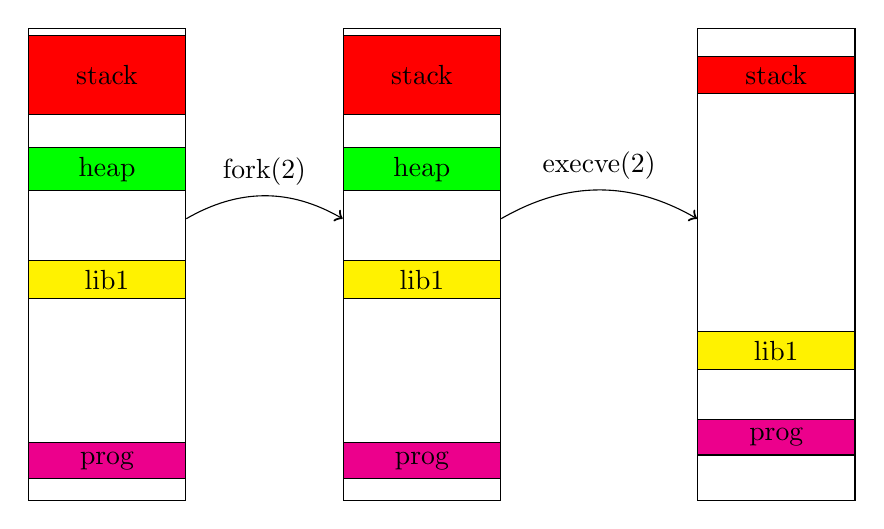
\begin{tikzpicture}
\path
    (0,0) node [draw,below,minimum width=2cm,minimum height=6cm] (p) {}
    +(0,-0.6) node [draw,minimum width=2cm,fill=red,minimum height=1cm] {stack}
    +(0,-1.8) node [draw,minimum width=2cm,fill=green] {heap}
    +(0,-3.2) node [draw,minimum width=2cm,fill=yellow] {lib1}
    +(0,-5.5) node [draw,minimum width=2cm,fill=magenta] {prog};
\path
    (4,0) node [draw,below,minimum width=2cm,minimum height=6cm] (f) {}
    +(0,-0.6) node [draw,minimum width=2cm,fill=red,minimum height=1cm] {stack}
    +(0,-1.8) node [draw,minimum width=2cm,fill=green] {heap}
    +(0,-3.2) node [draw,minimum width=2cm,fill=yellow] {lib1}
    +(0,-5.5) node [draw,minimum width=2cm,fill=magenta] {prog};
\path
    (8.5,0) node [draw,below,minimum width=2cm,minimum height=6cm] (e) {}
    +(0,-0.6) node [draw,minimum width=2cm,fill=red] {stack}
    +(0,-4.1) node [draw,minimum width=2cm,fill=yellow] {lib1}
    +(0,-5.2) node [draw,minimum width=2cm,fill=magenta] {prog};
\draw [->] (p) to [thick,bend left,edge label={fork(2)}] (f);
\draw [->] (f) to [thick,bend left,edge label={execve(2)}] (e);
\end{tikzpicture}
\end{frame}

\subsection{LibC Linking}
\begin{frame}{LibC Linking}
\includegraphics[width=\textwidth]{img/libc.ps}
\end{frame}

\subsection{LibC Relinking}
\begin{frame}{LibC Relinking}
\includegraphics[width=\textwidth]{img/new-libc.ps}
\end{frame}

\subsection{KARL Kernel Address Randomized Link}
\begin{frame}{KARL Kernel Address Randomized Link}
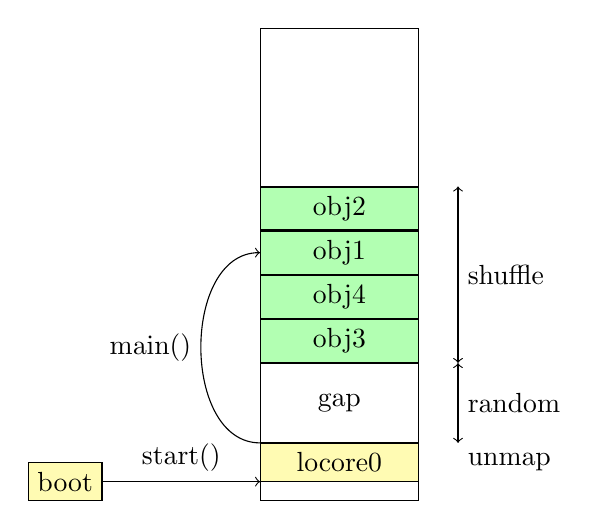
\begin{tikzpicture}
\path
    [minimum width=2cm,above]
    (0,0) node [draw,minimum height=6cm] (kernel) {}
    node (kerntext) {}
    (kerntext.north) node [draw,fill=yellow!30] (locore0) {locore0}
    (locore0.north) node [draw,minimum height=1cm] (gap) {gap}
    (gap.north) node [draw,fill=green!30] (obj3) {obj3}
    (obj3.north) node [draw,fill=green!30] (obj4) {obj4}
    (obj4.north) node [draw,fill=green!30] (obj1) {obj1}
    (obj1.north) node [draw,fill=green!30] (obj2) {obj2};
\draw
    (locore0.south west) [<-] -- node [above,midway] {start()}
    +(-2,0) node [anchor=east,draw,fill=yellow!30] (boot) {boot};
\draw
    (locore0.north west) [->] .. controls +(-1,0) and +(-1,0) ..
    node [midway,left] {main()} (obj1.west);
\draw
    (obj3.south east) +(0.5,0) coordinate (ostart)
    (obj2.north east) +(0.5,0) coordinate (oend)
    [<->] (ostart) -- (oend) node [midway,right] {shuffle};
\draw
    (gap.south east) +(0.5,0) coordinate (gstart)
    (gap.north east) +(0.5,0) coordinate (gend)
    [<->] (gstart) -- (gend) node [midway,right] {random};
\path
    (locore0.south east) +(0.5,0) coordinate (lstart)
    (locore0.north east) +(0.5,0) coordinate (lend)
    (lstart) -- (lend) node [midway,right] {unmap};
\end{tikzpicture}
\end{frame}

\subsection{Relink Time}
\begin{frame}{Relink Time}
\begin{itemize}
    \item libc, libcrypto, ld.so
    \begin{itemize}
	\item early boot
    \end{itemize}
    \item kernel
    \begin{itemize}
	\item install
	\item upgrade
	\item syspatch
	\item after boot
    \end{itemize}
\end{itemize}
\end{frame}

\subsection{Hide Kernel Addresses}
\begin{frame}{Hide Kernel Addresses}
\begin{itemize}
    \item -rwx------ root wheel /bsd
    \item fstat(1), netstat(1), ...
    \item /dev/kmem $\rightarrow$ \texttt{sysctl(2)}
    \item sysctl kern.allowkmem=1
\end{itemize}
\end{frame}

\section{SROP}

\subsection{SROP Signal Return Oriented Programming}
\begin{frame}{SROP Signal Return Oriented Programming}
\includegraphics[width=\textwidth]{img/srop.ps}
\end{frame}

\subsection{sigreturn(2) from Signal Handler}
\begin{frame}{sigreturn(2) from Signal Handler}
\includegraphics[width=\textwidth]{img/sigreturn.ps}
\end{frame}

\subsection{Signal Cookie}
\begin{frame}{Signal Cookie}
\includegraphics[width=\textwidth]{img/anti-srop.ps}
\end{frame}

\section{Spinoffs}

\subsection{LibreSSL}
\begin{frame}{LibreSSL}
\begin{itemize}
    \item keep OpenSSL 1.0 API
    \item fix bugs
    \item delete crap
    \item cleanup code
    \item backport features
    \item write documentation
\end{itemize}
\end{frame}

\subsection{OpenNTPD}
\begin{frame}{OpenNTPD}
\begin{itemize}
    \item avoid 40 CVE a year
    \item necessary features
    \item privilege separation
    \item reasonable accuracy
\end{itemize}
\end{frame}

\section{Compiler}

\subsection{Secure Compiler Defaults}
\begin{frame}{Secure Compiler Defaults}
\begin{itemize}
    \item clang 5.0.1, gcc 4.2.1
    \item PIE by default
    \item -fstack-protector-strong
    \item -fno-strict-aliasing
    \item -fno-strict-overflow
    \item -fwrapv
    \item no \texttt{malloc(3)} builtins
\end{itemize}
\end{frame}

\section{Conclusion}

\subsection{Questions}
\begin{frame}{Questions}
\begin{center}
\begin{tikzpicture}
\draw [font=\Huge] node {?};
\end{tikzpicture}
\end{center}
\end{frame}

\subsection{Links}
\begin{frame}{Links}
\begin{itemize}
    \item OpenBSD innovations
	{\small \url{https://www.openbsd.org/innovations.html}}
    \item deraadt@ slides about mitigations
	{\small \url{https://www.openbsd.org/papers/bsdtw.pdf}}
    \item man pages at {\small \url{https://man.openbsd.org/}}\\
	\texttt{pledge(2)
	kbind(2)
	sendsyslog(2)
	getentropy(2)
	getdtablecount(2)
	gcc-local(1)
	clang-local(1)
	random(3)
	malloc.conf(3)}
\end{itemize}
\end{frame}

\end{document}
